\documentclass{standalone}
\usepackage{tkz-fct}
\usepackage{tkz-euclide}
\usepackage{color}
\usepackage{amsmath}
\renewcommand*\familydefault{\sfdefault}
\usepackage{sansmath}
\sansmath
\definecolor{gray75}{gray}{0.75}
\begin{document}
 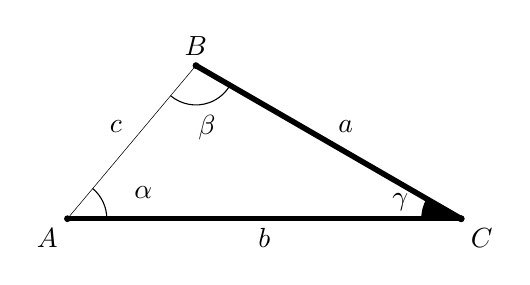
\begin{tikzpicture}[scale=1]
    \tkzDefPoint(0,0){A}
    \tkzDefPoint(5,0){C}
    \tkzDefTriangle[two angles = 50 and 30](A,C)
    \tkzGetPoint{B}
    \tkzDrawSegment(A,B)
    \tkzDrawPoints(A,B)
    \tkzDrawSegment[line width=2pt](A,C) 
    \tkzDrawSegment[line width=2pt](B,C)
    \tkzDrawPoints(C)
    \tkzFillAngle[fill=black, size=0.5](B,C,A)
    \tkzLabelPoints[below left](A)
    \tkzLabelPoints[above](B)
    \tkzDrawPoints(C)
    \tkzLabelPoints[below right](C)
    \tkzLabelAngle[pos=0.8, right](C,A,B){$\alpha$}
    \tkzLabelAngle[pos=0.8](A,B,C){$\beta$}
    \tkzLabelAngle[pos=0.8](B,C,A){$\gamma$}
    \tkzMarkAngle[size=0.5](C,A,B)
    \tkzMarkAngle[size=0.5](A,B,C)
    \tkzMarkAngle[size=0.5](B,C,A)
    \tkzLabelSegment[above right](C,B){$a$}
    \tkzLabelSegment[above left](B,A){$c$}
    \tkzLabelSegment[below](A,C){$b$}
\end{tikzpicture}
\end{document}
